\documentclass[preview]{standalone}

\usepackage[english]{babel}
\usepackage{amsmath}
\usepackage{amssymb}
\usepackage{tikz}
\usepackage{verbatim}
\usepackage{nicematrix}
\usepackage{fancyvrb}
\usepackage[hyphens]{url}

\usepackage{xcolor}
\usepackage{color}
\usepackage{colortbl}
\usepackage{xspace} % fix missing spaces after fancy commands e.g. \dagster
\usepackage{makecell}
\usepackage{fancyvrb}
\usepackage{tikz}
\usepackage{tikzscale}
\usepackage{pgfplots}
\usepackage{graphicx}
\usepackage{todonotes}
\usepackage{wrapfig}
%\usepackage{dingbat}
% to be able to draw some self-contained figs
\usepackage{tikz}
\usepackage{amsmath}
\usepackage{subcaption}
\usepackage[misc]{ifsym}
\usepackage{nicematrix}


\begin{document}

\begin{center}


\begin{figure}[!ht]
\centering
    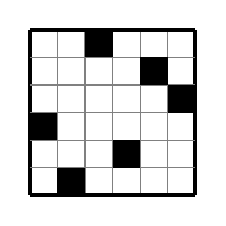
\begin{tikzpicture}[xscale=0.35, yscale=-0.35]
\draw[ultra thick] (0,0)--(0,6);
\draw[gray,thin] (1,0)--(1,6);
\draw[gray,thin] (2,0)--(2,6);
\draw[gray,thin] (3,0)--(3,6);
\draw[gray,thin] (4,0)--(4,6);
\draw[gray,thin] (5,0)--(5,6);
\draw[ultra thick] (6,0)--(6,6);

\draw[ultra thick] (0,0)--(6,0);
\draw[gray,thin] (0,1)--(6,1);
\draw[gray,thin] (0,2)--(6,2);
\draw[gray,thin] (0,3)--(6,3);
\draw[gray,thin] (0,4)--(6,4);
\draw[gray,thin] (0,5)--(6,5);
\draw[ultra thick] (0,6)--(6,6);

\fill [black] (2,0) rectangle (3,1);
\fill [black] (4,1) rectangle (5,2);
\fill [black] (5,2) rectangle (6,3);
\fill [black] (0,3) rectangle (1,4);
\fill [black] (3,4) rectangle (4,5);
\fill [black] (1,5) rectangle (2,6);

\end{tikzpicture}
%\caption{Costas array for $n=6$.}\label{fig:costas1}

\caption{An example Costas array}\label{fig:costas_subfigure}\label{fig:costas1}\label{fig:costas1}
\end{figure}



\end{center}

\end{document}
